\documentclass[10pt,a4paper]{memoir}
\usepackage{graphicx}
\usepackage{nth}
\usepackage{geometry}
\usepackage{subcaption}
\usepackage[colorlinks=false, allbordercolors={0 0 0}, pdfborderstyle={/S/U/W 1}]{hyperref}
\usepackage{listings}
\usepackage{pythonhighlight}
\usepackage{parskip}
\usepackage{booktabs}
\usepackage{siunitx}
\usepackage{mhchem}

\setlrmarginsandblock{2cm}{2cm}{*}
\setulmarginsandblock{2cm}{*}{1}
\checkandfixthelayout


\setlength{\parskip}{0.3cm}
\renewcommand{\thesection}{\arabic{section}}
\renewcommand{\familydefault}{\rmdefault}

\title{{\Huge{Data Analysis using Python}}\\
{\large{A Guide for Chemistry Undergraduates}}}
\author{James D. Pickering\thanks{james.pickering@leicester.ac.uk}\thanks{pickering.jamesd@gmail.com}}
\begin{document}
\maketitle
The purpose of this short course is two-fold. First and foremost, it is designed to enable undergraduate chemists to use Python for data analysis and to allow them to create high-quality (publication standard) figures for use in reports and dissertations. Secondly, it will help to address the widespread programming illiteracy amongst undergraduate students, empowering them to become more confident in use of programming languages as they progress through an undergraduate course.  

The programming language used throughout will be \href{www.python.org}{Python}, with a focus on \href{www.matplotlib.org}{Matplotlib} from the \href{www.scipy.org}{SciPy} suite of packages (a set of packages for mathematicians, scientists, and engineers). 

\section*{Why Python?}
An obvious question that will arise is: `Why use Python and not a more familiar computer program?'. While it is possible (and simpler, in the short term) to use proprietary software such as Microsoft Excel or Origin to perform data analysis and produce figures, using Python has some distinct advantages:
\begin{enumerate}
	\item \emph{Flexibility} - As it is an open-source programming language, Python (and specifically the SciPy suite of packages) is infinitely more flexible than proprietary software such as Excel or Origin. This is especially useful for scientists as often we want to do non-standard things to our data. 
	\item \emph{Cost} - Python and all related packages are \emph{open source} and \emph{free}, in contrast to software such as Excel or Origin, and even in contrast to other programming languages such as MATLAB or Wolfram Mathematica. This means that no site licences are required, and any student can install it on any computer and practice wherever they are.
	\item \emph{Programming Literacy} - Becoming literate in any programming language makes it exponentially easier to learn other programming languages. Becoming comfortable with Python will make using any other language (such as MATLAB or Mathematica) easier, meaning that you can spend more time thinking about the science, and less time thinking about the programming.
\end{enumerate}

Are there any downsides? There will certainly be a (hopefully not too steep) learning curve initially - but this course aims to make that as pain-free as possible. The huge flexibility inherent in an open-source language such as Python can also make things confusing as there are often multiple ways to achieve the same result! With experience this becomes easier to navigate, and the material used in this course is intended to be as self-consistent as possible. 

Hopefully this convinces you that fluency in a programming language is a worthwhile thing to work towards. With practice, figures such as those shown below (taken from my published articles) can be easily created - without giving any money to Microsoft or Originlab! 
\begin{figure}[h]
\centering
	\begin{subfigure}[b]{0.45\textwidth}
		\includegraphics[width=\textwidth]{example_fig1.pdf}
	\end{subfigure}
	\quad
	\begin{subfigure}[b]{0.35\textwidth}
		\includegraphics[width=\textwidth]{example_fig3.pdf}
	\end{subfigure}
\end{figure}
\begin{figure}[h]
	\centering
	\includegraphics[width=\textwidth]{example_fig2.pdf}
\end{figure}

\section*{Before We Begin}
Before we start actually using Python for things, it's useful to quickly discuss how this course is designed to be used. 

It is designed to be fairly self-contained, so you should be able to follow most of it just from the information in this document. However, if you're confused about how to achieve something (and this happens to everyone, even experienced users!), \textbf{then the best place to find help is online}. One of the great things about Python and the SciPy packages is that there is a \textbf{huge} amount of online documentation (see, for example, \url{https://matplotlib.org/contents.html}). On top this documentation, you can nearly always find the answer to any problem you have on StackOverflow (\url{https://stackoverflow.com/}). 

In my experience the best way to learn and use Python is to have it open next to a web browser so you can easily google things when you get stuck. 99.99\% of the time, simply googling the problem you have will lead you to a solution - there is a \emph{huge} amount of help available online. Learning by using it, and googling any issues, is how most people learn to use programming languages (it's how I did it!) - and definitely works. This document should just help provide a structure to the learning process.
\vspace*{\fill}

\section{Installation}
N.B. IN ANY INSTALLATION, MAKE SURE TO INSTALL PYTHON 3.x AND NOT PYTHON 2.7. THE MOST RECENT RELEASE IS PYTHON 3.7.2 AT TIME OF WRITING.

In general, following the advice at \url{https://docs.spyder-ide.org/installation.html} is a reasonable place to start.
\subsection{MS Windows and Mac OS}
Python, together with Matplotlib, SciPy, NumPy, and many other packages can be easily installed on MS Windows or Mac OS using \href{https://www.anaconda.com/download/#download}{Anaconda}. This installation installs all the relevant software, including the \href{www.spyder-ide.org}{Spyder} IDE that will be used throughout this short course. It also includes the \href{www.qt.io/qt-for-python}{Qt} packages that are required to show plots and help the graphical functionality.

Anaconda is quite a big file as it contains all the packages you'll need and lots of different development environments. It might take a while to download and install. Once it's installed, you can just launch Anaconda Navigator from the start menu (normally ina folder called anaconda3), and then from there launch Spyder.

When you first launch spyder, and before starting any programming, it's a good idea to go into Tools $>$ Preferences $>$ IPython Console $>$ Graphics and change the graphics backend from `inline' to `automatic'. This just means that any figures you create are opened in separate windows rather than in the terminal - it makes it a lot easier to see and analyse things.
\subsection{Linux}
The quickest way to get up and running on linux is also to download \href{https://www.anaconda.com/download/#linux}{Anaconda}. This contains all the packages you need to use (and a lot that you won't!). You can also use \texttt{apt-get} or similar to install each component separately if you'd prefer to only install the packages you want. I'm assuming that if you're running linux (like me) then you're probably able to navigate this installation yourself!  

\section*{How to Use This Document}
I would suggest having this document open while you're using Spyder, and typing in the example codes and running them to check that you produce the same figure as is shown in each subsection.

The data files, figure files, and any other required files (e.g. images that are plotted) can be found on the associated GitHub page at \url{https://github.com/james-d-pickering/data-analysis-with-python}. Here all the codes presented in this document are also available for download, and versions of them with additional comments to aid understanding. The source code for this \LaTeX~document can also be found there.


\newpage

\section{Using Spyder - Basic Python}
Spyder is an Integrated Development Environment (IDE) - this means it consists of both a text editor (where you will write your code), and a console (where you run your code and see the output). It has a lot more functionality than just this - but these are what we will primarily use in this course. 

You can either write commands directly into the terminal (easy but limiting as you can only do one thing at a time), or can write them in the editor to run as a block. We will always use the editor. As a simple first example, try typing the following into the editor and then pressing run (F5, or click the green `play' arrow - note you may have to save your script before it will run). \inputpython{hello_world.py}{1}{2}

In the terminal you should now see the words "Hello, World!". That was your first Python program! You can find the source code for this (and all other programs shown in this course) online on github \url{https://github.com/james-d-pickering/data-analysis-with-python}. In general the programs are online both as they appear in this document and with comments added to each line for further explanation.

You should now be comfortable with writing things in the editor and running them, seeing the output in the console. We will mainly `learn as we go' - learning about the various bits of functionality as we need them. However, there are a few things worth learning before we start. See the program below. \inputpython{basic_python.py}{1}{18}

Running the program basic\_python.py should produce three lines of console output:
\begin{lstlisting}
Hello, World!
Hey!
3.14159 Hey!
\end{lstlisting}
We should now be familiar with the concept of comments (lines starting with \# which are not run in the console and only serve to describe the surrounding code), and of variables. The final thing to define is what is meant by the terms \emph{function} and \emph{argument}. A \emph{function} is a command that the computer understands to make it do something - in the above code, \texttt{print} is a function. The \emph{argument} of a function is the input you feed it to tell it how to behave - in the above code, the string \texttt{"Hello, World!"} was an argument.  

We will now start to actually use matplotlib and make some figures!
\newpage

\section{Basic Plotting using Matplotlib}
Matplotlib (from MAThematical PLOTting LIBrary) is a package contained in the SciPy (SCIentific PYthon) set of packages. There area few different packages contained in this set, and you can see them all at \url{www.scipy.org}. We will only use three of the packages: SciPy and Matplotlib (already mentioned), together with NumPy (NUMerical PYthon). These packages provide a huge variety of functions and commands useful to us as scientists. Let's set up the workspace.

\subsection{Setting up a Workspace}
As we will be using NumPy, SciPy, and Matplotlib almost exclusively, we need to import them every time we write some code. Importing them means telling the computer that we're about to use these packages, so it should be ready to use the functions contained within them. Accordingly, the first three lines of code in any of our programs will be as follow. \inputpython{importing_packages.py}{1}{3} 

The first two lines are simple - we import the package `numpy' and call it `np' (this just saves us writing `numpy' every time we want to use it - more later), and do the same for `scipy'. The third line is importing matplotlib, but notice that we actually import `matplotlib.pyplot' - what this is saying is `import the sub-package from matplotlib called pyplot'. Matplotlib is a big package, and we only want to use the pyplot part of it (at the moment), to help us with plotting. We import it as `plt' for similar reasons to above. 

\subsection{First Plot}
Let's plot a sine function. To do this, we will use the following code. 

\begin{minipage}{0.48\textwidth}
	\inputpython{first_plot.py}{1}{17}
\end{minipage}
\quad
\begin{minipage}{0.48\textwidth}
		\centering
		\includegraphics[width=\textwidth]{first_plot.png}
\end{minipage}

The first three lines we've already covered. The next line is a command that closes all our open plots (this will save us from opening too many windows at once). 

The following three lines are defining three variables: pi (self-explanatory), $x$, and $y$. The $x$ variable is defined using the function \texttt{np.linspace} - the arguments are \texttt{linspace( start, end, number of points)} - so we are creating a list of 50 equally spaced numbers, starting at 0 and ending at $2\pi$\footnote{We write \texttt{np.linspace} because the \texttt{linspace} function is part of the \texttt{numpy} package, which we imported as \texttt{np} in line 1.}. This is what is known as a \emph{vector}, and is an important thing to understand. Whenever we now use the variable $x$, we are referring to this 50 element long vector.

Turning to $y$, this is defined using the function \texttt{np.sin} to be the sine of $x$, as should be familiar. Accordingly, $y$ is now a 50 element long vector, where each each element is the sine of the corresponding element in vector $x$. To take a concrete example, the first element of $x$ is zero, and the first element of $y$ would be $\sin (0)$, which is also equal to zero. Have a play around with this until you feel comfortable with what's happening.

The remainder of the lines make the plot. (Almost) every line starts with the \texttt{plt} command, as they are using functions from the \texttt{matplotlib.pyplot} package. Each line is fairly self-explanatory, but we will quickly run through them. The first line is just creating a blank figure, which we are calling \texttt{fig} - so we can easily refer to it. The second line is using the function \texttt{plt.plot} to plot a line graph of $x$ against $y$. The remainder of the lines simply make this graph look prettier! The function \texttt{plt.xlim} sets the limits of the $x$ axis - here between $0$ and $2\pi$. The functions \texttt{plt.xlabel} and \texttt{plt.ylabel} set the x- and y- axis labels, respectively. The function \texttt{plt.title} sets the title. The function \texttt{plt.grid} turns the gridlines on or off. Finally, the function \texttt{plt.savefig} saves the current plot as ``first\_plot.png" in the same directory as the plotting program.  

\noindent If it all ran smoothly, the resulting plot should look like the plot next to the code above!

\noindent \textbf{Exercises 1}

Use matplotlib to plot graphs of the following:

\begin{enumerate}
	\item $\cos(x)$ between zero and $\pi$ radians.
	\item $\cos(x), \sin(x)$, and $\sin^2(x)$ between 0 and $2\pi$ on the same plot (bonus: can you make each one a different colour?).
	\item $\sin(x)$ and $\cos(x)$ on the same plot from 0 to 360$^\circ$ - with the $x$ axis in degrees.
\end{enumerate}
\newpage

\section{Different Types of Plot}
So far we have seen how to make simple line graphs. This is nice, although often we will want to make different kinds of plots. The process is much the same, just using different functions. We will try a few of them now, and show some ways of entering data at the same time.

\subsection{Scatter Plots}
A Python code to make a simple scatter plot is given below. 

\begin{minipage}{0.48\textwidth}
	\inputpython{scatter_plot.py}{1}{18}
\end{minipage}
\quad
\begin{minipage}{0.48\textwidth}
		\centering
		\includegraphics[width=\textwidth]{scatter_plot.png}
\end{minipage}

Most of this is familiar now! The main difference is in how we have defined our $x$ and $y$ variables - we haven't used the \texttt{np.linspace} function to make our vector of points, we've put the points in directly by using \texttt{np.array}. Using \texttt{np.array} is a simple way to enter data, and is easy if you don't have many points, or can't auto-generate them (i.e. if you measured them by hand in the lab). 

Having defined these, the rest is all fairly familiar. The only difference is that instead of using \texttt{plt.plot} we've used \texttt{plt.scatter}. The result should look like the figure next to the code above. You could even use both \texttt{plt.plot} and \texttt{plt.scatter} in the same code and get both the points and the line connecting them - try it out!

\subsection{Histograms}
A Python code to make a simple histogram is given below. The histogram will show the heights of some imaginary trees, and tells you how many trees there were in different height ranges.

\begin{minipage}{0.48\textwidth}
	\inputpython{histogram.py}{1}{18}
\end{minipage}
\quad
\begin{minipage}{0.48\textwidth}
		\centering
		\includegraphics[width=\textwidth]{simple_histogram.png}
\end{minipage}

Again it's mostly familiar - but we have loaded the data in in a different way again. Now we have loaded the data from the text file \texttt{heights.txt} (this file is found in the folder \texttt{/data\_files/}). Loading data from files is probably the most common way of doing things. In this case, it's very simple as our file only contains one column of numbers (open it and see), but we will do some more complex examples later.

The other difference is we have now use the \texttt{plt.hist} command. The arguments this takes are our list of heights (that we loaded from the file \texttt{heights.txt}), and also an extra argument \texttt{bins=height\_bins}. This argument is specific to the \texttt{plt.hist} function. To plot a histogram the computer needs to know both the data, and what size bin to use - if you look at the histogram it is showing you how many trees are between 3 and 4 feet, then between 4 and 5 feet, and so on. The \texttt{bins} argument tells you how fine or coarse these bins are. We've defined 1 foot wide bins, but it could be coarser (2 feet wide) or finer (0.5 feet wide). Try and play with the array that defines \texttt{height\_bins} and see how it affects the resulting plot.

You'll also notice that now we only have gridlines turned on for the $x$ axis - how did we do this?

\subsection{Pie Charts}
The code for a simple pie chart is below. By now this should all be getting familiar, so let's add some complexity.

\begin{minipage}{0.48\textwidth}
	\inputpython{pie_chart.py}{1}{15}
\end{minipage}
\quad
\begin{minipage}{0.48\textwidth}
		\centering
		\includegraphics[width=\textwidth]{pie_chart.png}
\end{minipage}

We load the data using the text file \texttt{pie\_chart.txt}, as before. We now need to define two other variables - \texttt{pie\_labels} and \texttt{explode} - to let us plot the pie chart nicely. The first of these is, as it says, giving a label for each section of the pie chart - these labels are in the same order as the data in \texttt{pie\_chart.txt}. The second of these is a bit tricker, but allows us to explode one segment of the pie chart so it can be seen more clearly - looking at the figure it is clear that the segment labelled "Liberal Democrat" is exploded out of the chart. The \texttt{explode} variable tells Python how much to explode each segment by - zero for all segments except the Liberal Democrat segment.

The rest just plots the pie chart! But we've added some new things. Firstly, you'll see that the function \texttt{plt.pie} is taking some extra arguments, not just \texttt{seats} and \texttt{labels}. We also have to pass it the \texttt{explode} array, to tell it to offset one segment, and we turn shadows on using the \texttt{shadow} argument so it looks more 3D. The \texttt{startangle} argument just rotates the pie chart so it looks nice - play with it and see how it works!

We've also added the line \texttt{plt.axis("equal")}, this simply forces the figure to be a square, if it isn't there then the figure is rectangular which squashes the pie chart and makes it look elliptical. The final change is making the font of the title bigger - can you see where that has changed?
\newpage

\subsection{Image Data}
The final example we'll consider in this section is if you want to plot an image - this could be a photo (to illustrate something) or it could be some experimental data like an ion image, or a microscope image. Fortunately, this is really straightforward in matplotlib - provided we have our image in the correct format. Let's try using a photo first, the following code will produce a picture of a blue tit that I took from my bedroom window (the photo file can be found in \texttt{/data\_files/}).

\begin{minipage}{0.48\textwidth}
	\inputpython{photo_plot.py}{1}{12}
\end{minipage}
\quad
\begin{minipage}{0.48\textwidth}
		\centering
		\includegraphics[width=\textwidth]{photo_plot.png}
\end{minipage}

The first difference you'll notice is that we had to load an extra package - \texttt{matplotlib.image}. This package contains all the tools for image manipulation, and we imported it as \texttt{mpimg} for brevity. We then used the function \texttt{mpimg.imread} to turn the png file into an $N\times M$ array, where $N$ and $M$ are the the number of pixels wide and high the image is, respectively. 

It's then very easy to plot the image, just use \texttt{plt.imshow(image)}. The penultimate line \texttt{plt.axis("off")} simply turns off the axis numbering and labelling, so we only see the photo.

However, what if what we want to plot isn't a colour photograph (with different RGB values for each pixel), but is just an array of pixels that all have different intensities (i.e. a black and white photo, or a photo from something like an electron microscope or imaging spectrometer)? In these situations, it's often useful to be able to alter the colour map and intensity of the image to highlight important features. We can approximate this situation with our blue tit using the following code. 

\begin{minipage}{0.48\textwidth}
	\inputpython{image_plot.py}{1}{16}
\end{minipage}
\quad
\begin{minipage}{0.48\textwidth}
		\centering
		\includegraphics[width=\textwidth]{image_plot.png}
\end{minipage}

Here, we have now defined \texttt{lum\_image} as being simply one colour channel of our original RGB photo. Now our image is essentially just the same $N\times M$ array, but with each pixel being assigned a value from 0 to 1 depending on how bright it is (lower values darker, higher values brighter). When we plot it now, we can assign a colourmap using the argument \texttt{cmap}, which determines which colours are used to plot our image. The current colourmap is \texttt{inferno}, but try others, such as \texttt{viridis, hot, jet} or \texttt{greys}. We have also used the arguments \texttt{vmin} and \texttt{vmax} to constrain the colourmap - 0 and 1 are the default values, but try changing them (e.g. to 0.3 and 0.6) and see how the image changes. 

The final thing we've done is use the function \texttt{plt.colorbar} to add a colour bar onto our image - so we can see which colours correspond to what in terms of intensity. This would be useful if (for example) brighter areas indicated high intensity signal (or something similar).

\subsection{The \texttt{plt.savefig} Function}
Before we continue, there is one quick thing that deserves it's own section, and that's the \texttt{plt.savefig} command. So far, we have just used this as \texttt{plt.savefig(`filename.png')} - this is great, but sometimes we will want to save things in different file formats, or change other things about how the figure is saved. A real-world example of this is if you are making a figure for a poster, so need it in high resolution for large printing; or if you are submitting a figure to a journal and they require a specific file format.

We can change the file type simply by changing the file extension in our filename, for example to \texttt{.pdf} instead of \texttt{.png}. We could also write \texttt{plt.savefig(`filename',format=`pdf')} to achieve the same thing. I'd suggest generally using PNG or PDF files wherever possible, but it's up to you. 

Other useful arguments we can pass to \texttt{plt.savefig} include: \texttt{dpi=number}, which sets the dpi (dots per square inch) of the figure. Generally at least 150 dpi is used, and 300 dpi should be sufficient for most things. For large printing of figures then using 600 or 1200 can be useful - or if you have a lot of detail that needs to be seen. You can also add \texttt{transparent=True} which makes the background transparent rather than white (useful if overlaying on a coloured background). There are others too - have a google!

\noindent \textbf{Exercises 2}
\begin{enumerate}
	\item Plot the ultraviolet absorption spectrum of benzene stored in the data file \texttt{`benzene\_UV\_spectrum.txt'}. The wavelength is in the first column and the absorption in the second. Plot it with both the data points and a line connecting them between 120 and \SI{190}{\nano\metre}. Note that the magnitude of the absorption data points is tiny, you may need to scale them to see things! 
	\item Lead has four stable isotopes. Plot a pie chart showing the relative abundance of each, exploding out the slice corresponding to the second least abundant.
	\item The file \texttt{`molecular\_speeds.txt'} contains a random sampling of the speeds of 1000 different nitrogen molecules at room temperature. Plot these a histogram. What distribution should the speeds fit? Can you plot this distribution as a smooth line over the histogram?
\end{enumerate}
\newpage

\section{Beautifying Plots}
Now we understand how to make a variety of different plots, and in the last few examples we've played a bit with customising things like font sizes. What we would like to be able to do is to have a lot more flexibility, and change things like colours, line styles, marker styles, etc... Helpfully, this is mostly just a case of passing additional arguments into commands like \texttt{plt.plot} which control such things. See the figure below for an example of this. The code for this is significantly more complex and would be cumbersome to place in line here, so instead try and open it (\texttt{fancy\_plot.py}) in Spyder and go through it line-by-line to see if you understand it. Remember there is a version with line-by-line comments if you don't understand anything!
\begin{figure}[h!]
	\centering
	\includegraphics[width=0.9\textwidth]{fancy_plot.png}
\end{figure}

The additional arguments we pass to \texttt{plt.plot} here are referred to as \texttt{kwargs} (short for KeyWord ARGumentS) - the nice thing about these is that a) they are often the same for many different functions, and b) you can often guess what they will be. For example, if I wanted to change the style of the line on a plot (from solid to dashed, for example), I would add the kwarg \texttt{linestyle='--'}. Other examples of common kwargs are \texttt{color, linewidth, markersize, alpha, fontsize,} and \texttt{fontfamily}. Not every kwarg is compatible with every function (\texttt{plt.plot} doesn't have the kwarg \texttt{fontsize}, for example) - but a lot of them are general.

A final note on colours in matplotlib. To add a colour to something, use the kwarg \texttt{color=`your colour'} (note american spelling). You can use a simple string like \texttt{`black'}, or \texttt{`blue'}; or you can use the hex RGB code like \texttt{`\#0F0F0F'}. You can even use one of the \href{https://xkcd.com/color/rgb/}{954 most common RGB monitor colours, as decided by xkcd}, by using the name from the linked page prefixed with \texttt{xkcd:}, such as \texttt{color=`xkcd:sickly green'}. Have a play around with it and get the hang of how it works. 
\newpage

\newpage
\section{Multiple Plots}
The last part of this introductory course will be about plotting multiple graphs in the same figure. This is useful if you need to include several different sub-plots in one larger figure for publication (as was shown in the example plots at the start), or if have experimental results that can each be plotted as a graph, but you want to show how the graphs change as you change one variable (for example). 

Thankfully, this is also quite straightforward using matplotlib - using the module \texttt{gridspec}.

\subsection{Using Gridspec}
The way Gridspec works is by splitting the figure into an $n\times m$ grid, and allowing a separate \textit{subplot} to be placed in each segment of the grid. A subplot functions in exactly the same way as all of the plots we've previously seen, but we will now have multiple subplots in one figure. \inputpython{multiple_plots.py}{1}{44}

\begin{figure}
	\centering
	\includegraphics[width=0.9\textwidth]{multiple_plots.png}
\end{figure}

You can see here we have added a new line to our preamble, loading \texttt{matplotlib.gridspec} as \texttt{gs}. We then define our grid using the function \texttt{gs.GridSpec}, which takes four arguments. The first two define how many rows and columns our grid spans, and the next two define the spacing between the columns and the rows respectively (bonus question: what units is this spacing given in?). Then, for each space in the grid, we produce a \emph{subplot} using the command \texttt{plt.subplot}.

Subplots function in the same way as when we would write \texttt{plt.figure}, but now something slightly different is happening in that we call each subplot \texttt{ax1,2,3...}. This is because strictly each subplot creates a set of \textbf{axes} at each location in the grid, and we plot things on those axes. We choose which element of the grid the axes are created in with the \texttt{grid[n,m]} argument passed to \texttt{plt.subplot}. In Python, lists are created with indexes \textbf{starting at zero, so the first element is (0,0)} - this is the same as languages like C or C++, and different to languages like MATLAB or Fortran (where the first element is (1,1)). So the first plot in our grid (top left) is defined as \texttt{grid[0,0]}. You should then see how we can access the top right plot (\texttt{grid[0,1]}), and we make the bottom plot span across two grid cells using \texttt{grid[1,:]} - the colon here means `span across all possible cells'. Play with this until you have a feel for how it works. 

The rest of the code is fairly similar to what we've already seen. We've now added in a few extra things, like moving the labels on an axis to the right hand side of a plot, and plotting one graph with two different y axes - but a lot of this should be self-explanatory or easy to figure out yourself by now. Two important functions we've added are the \texttt{plt.text(x, y, str)} function, which plots a text string \texttt{str} at the coordinates $x, y$ (the coordinates are defined in terms of the axes in the figure). Additionally, the \texttt{fig.suptitle} command, which adds an overall title to the plot - using \texttt{plt.title} with gridspec will only add the title to a specific subplot. 

Finally, in this instance the result we get just from using \texttt{gridspec} is nice and looks good. However, sometimes \texttt{gridspec} can be a real pain and you end up getting weird aspect ratios, axis labels that protrude outside of the figure, or overlapping subplots. In these instances, what you should do is \textbf{force} python to make the figure a specific size. You do this by altering \texttt{plt.figure()} to \texttt{plt.figure(figsize(n,m))}, where $n$ and $m$ are the dimensions of the figure \textbf{in inches} - Americans made this package.. If you come across an example in the exercises below where this seems to be an issue, try and force the figure to be a specific size in the way just described - it helps! You should also make sure that if you change the \texttt{figsize} command that you \textbf{look at the final .png file, not the pop-up window that Spyder produces} - often these two things aren't the same.  

\noindent \textbf{Exercises 3 - Harder!}
\begin{enumerate}
	\item Plot the three main trigonometric functions, $\sin, \cos$, and $\tan$ side by side on 3 different subplots, between $-2\pi$ and $2\pi$. Watch out for clipped axis labels! 
	\item Make a $3\times 3$ Andy Warhol inspired picture of my blue tit (or another photo), with each one plotted using a different colour map. 
	\item (Bonus for serious punters) The same as above, but done using a \texttt{for} loop. I haven't covered this, but it's google-able!
\end{enumerate}
\newpage
\section{Concluding Remarks}
If you've completed all the preceding sections, you should be fairly competent and able to continue using matplotlib to present yor data and make informative (and beautiful) figures. There is a lot more functionality than what has been covered here, and there's enough documentation online for you to be able to pick most of that up reasonably quickly once you're familiar with the basic syntax. Remember you can find all the bits of code used here, with comments, on the associated GitHub page: \url{https://github.com/james-d-pickering/data-analysis-with-python}. Comments and criticism welcome at \texttt{pickering.jamesd AT gmail DOT com}.

Happy Python-ing!

\begin{figure}[h!]
	\centering
	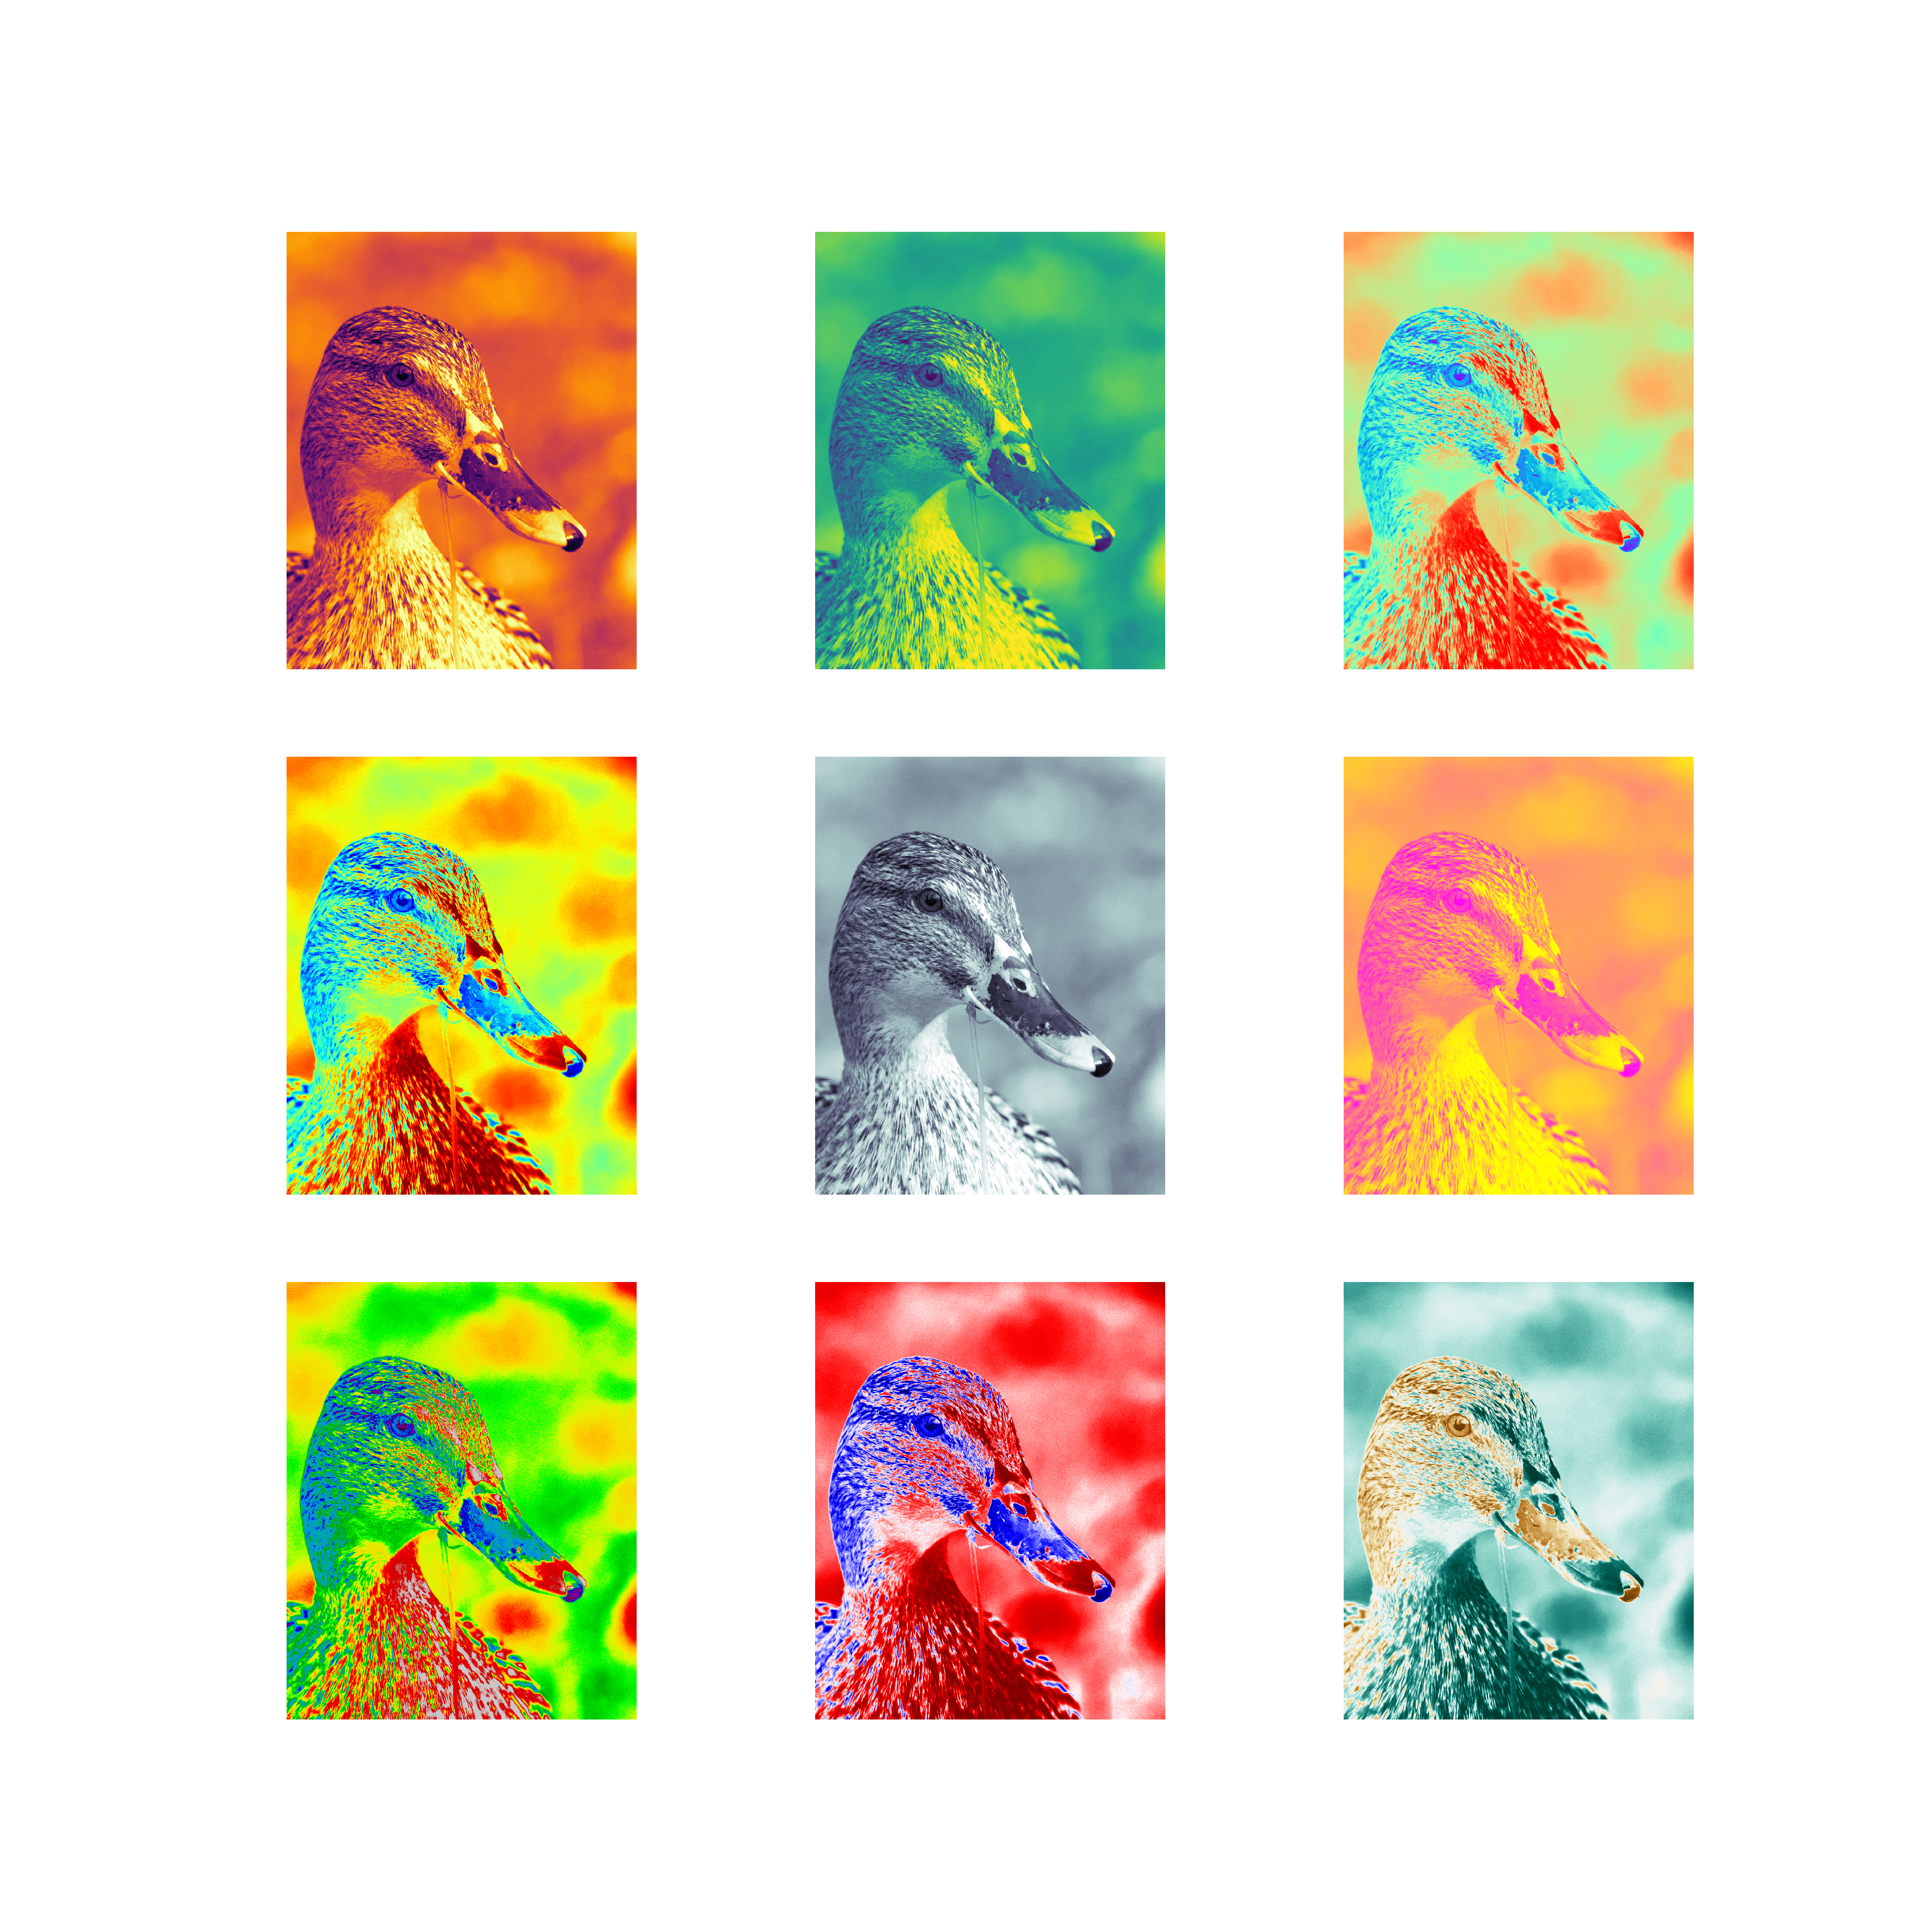
\includegraphics[width=\textwidth]{duck_warhol.png}
\end{figure}










\end{document}

